\documentclass[11pt]{article}

%\usepackage{fullpage}          %sorgt dafr, dass alle Rnder 1 inch breit sind
\topmargin=-1.0cm
\textheight=23cm
\evensidemargin=-1.0cm
\oddsidemargin=-1.0cm
\textwidth=19cm

\setcounter{secnumdepth}{-1}    % suppress numbering of sections


\usepackage{amsmath}
\usepackage{amssymb}             % for mathbb
\usepackage{graphicx}
\usepackage{float}               % for positioning graphics via [h!]
\usepackage{hyperref}            % for hyperlinks
%\usepackage{subfig}
\usepackage{caption}
\usepackage{subcaption}

%% header/footer stuff does complain on windows:
%\usepackage{fancyhdr}           % for headers and footers
%\pagestyle{fancy} 
%\rhead{}
%\rfoot{\htmladdnormallink{www.rs-met.com}{http://www.rs-met.com}} 

% set the footer:
%\rfoot{article available at: http://www.rs-met.com}



\begin{document}

% formatting options:
\parindent=0in
\parskip=0pt

\pagenumbering{arabic} \setcounter{page}{1}

% main body:
\begin{center}
\section{GNUPlotCPP - User Manual}
\end{center}

\section{Introduction}
GNUPlotCPP is a C++ library for interfacing with GNUPlot directly from C++ code. The idea behind it is that, during research-and-development phases of programming, you may want to visualize some data that occurs somewhere inside your code. Or you may want to write some experimental code that deliberately produces test data for visualization. So, basically, GNUPlotCPP is a tool for experimentation, development and debugging of C++ code. It may also be useful for creating plots for inclusion into technical documentations of your algorithms and code. For example, you may want to plot the content of two arrays of length \texttt{N} as y-values in a single plot (say, for comparison purposes), using the array indices as x-values. With GNUPlotCPP, you could do this by inserting:
\begin{verbatim}
GNUPlotter p;
p.plotArrays(N, myArray1, myArray2);
\end{verbatim}
into your code. Here, \texttt{myArray1} and \texttt{myArray2} would be arrays of values (\texttt{int}, \texttt{float} and \texttt{double} types are supported). If you are familiar with languages like MatLab, you will notice that this is not quite unlike the built-in plotting facilities there. Visualizing data is an important tool in the development of algorithms and C++ is lacking in this area. This interface to GNUPlot is an aim at filling this gap. The main objective is to bring MatLab-like plotting capabilities into a C++ coding environment. As another example, maybe you want to plot one of your self written functions for a range of argument values, in order to convince yourself, that the function produces the expected output and/or to learn about how the output actually looks like if you have no idea. A simple code fragment could look like:
\begin{verbatim}
GNUPlotter p;
p.plotFunctions(1000, -5.0, 10.0, &myFunction);
\end{verbatim}
for plotting your function \texttt{myFunction} with argument values from \texttt{-5} to \texttt{10} (using \texttt{1000} sampling values between the limits). Your function should in this case take one parameter and return a value of the same type (again, \texttt{int}, \texttt{float} and \texttt{double} types are supported), like - for example - the standard-library function \texttt{sin} which takes a \texttt{double} parameter and returns a \texttt{double} value. Here, you could also have passed multiple functions (up to 10) which would then be shown as several graphs in a single plot. Note that via the \texttt{\&} operator, you are  passing a function pointer to \texttt{myFunction} to the \texttt{plotFunctions} member function of the \texttt{GNUPlotter} class.

\section{How does it work?}
GNUPlot, by itself, is a command line driven plotting application. Once it is running, you can enter commands at the prompt to let it plot functions or display data from files in various ways. The plots will be shown in a separate window. In addition to accepting realtime input from a command line prompt, GNUPlot may also read a batch file that contains a sequence of commands. You can specify that batchfile as commandline parameter when you launch GNUPlot. The batchfile itself may then contain all the commands that control, which data is used (for example, it tells GNUPlot to read data from one or more datafiles) and how the data should be interpreted and presented. The \texttt{GNUPlotter} class uses this batchfile mechanism to control the presentation of the data and it uses the datafile mechanism to pass the actual data to GNUPlot. When you use it like:
\begin{verbatim}
GNUPlotter p;
p.plotFunctions(1000, 0.0, 10.0, &sin, &cos);
\end{verbatim}
the following things happen:
\begin{enumerate}
	\item the \texttt{GNUPlotter} object \texttt{p} is created
	\begin{enumerate}
		\item a datafile and commandfile are intialized
		\item a couple of default commands are written into the commandfile in order to achieve the desired default plotting behavior
	\end{enumerate}
	\item	\texttt{plotFunctions} is called on \texttt{p}
	
	\begin{enumerate}
		\item the actual data is generated (i.e. the x-axis values and y-axis values for the two functions) and written into the datafile
		\item GNUPlot is invoked and instructed to read in the commandfile which in turn sets up the plotting options and instructs GNUPlot to read the datafile and plot the data in it.
	\end{enumerate}
\end{enumerate}
The general mode of operation is: let your code generate the data that you want to visualize, use suitable functions of the \texttt{GNUPlotter} class to add your data to a GNUPlot datafile, use other functions to generate a GNUPlot commandfile, run GNUPlot. The call of \texttt{p.plotFunctions} wraps all of these steps into a convenient single-line function call. Such convenience functions exist for some of the more common tasks, but you have also access and control over the lower level steps in order to harness the complete feature set of GNUPlot itself..

\subsection{Preliminaries}
In order to make that work, you obviously need to have GNUPlot installed on your computer. Somewhere in the code, there's a \texttt{std::string} variable \texttt{gnuplotPath} for the installation path. The variable is initialized in the constructor of the \texttt{GNUPlotter} class and its value is set to GNUPlot's default installation path on Windows via the line:
\begin{verbatim}
gnuplotPath = "C:/Program Files/gnuplot/bin/gnuplot.exe";
\end{verbatim}
If your installation path is different, you can change the path there. For the temporary data- and commandfile, the paths are set up as:
\begin{verbatim}
dataPath    = "E:/Temp/gnuplotData.dat";
commandPath = "E:/Temp/gnuplotCommands.txt"; 
\end{verbatim}
The directory where the files will be written into \texttt{(E:/Temp} in this case), has to exist on your machine. If you want to have the files written into a different directory, change the code there (beware that it should not contain any whitespaces). Now, you only need to include \texttt{GNUPlotter.h} somewhere in your code, from where you want to use it, add the \texttt{GNUPlotter.h, GNUPlotter.cpp} files to your IDE project and you should be ready to go.


\section{Customization of Plots}
%make sections for plotting styles and line styles
These examples above are the simple cases, where we didn't control any plotting options manually. Instead, we just relied on the automatic default behavior provided by the GNUPlotter class. For simple debugging and experimentation scenarios, this is often good enough. However, if you need more control over the way, in which the data is presented, you can call some setup functions in between the creation of the object, and the function call that eventually invokes GNUPlot and initiates the actual plotting. For example, calling
\begin{verbatim}
p.addCommand("set xrange[-5:5]");
p.addCommand("set yrange[-1:10]");
\end{verbatim}
has the effect of setting the range of the x-axis to -5...5 and the range of the y-axis to -1...10 instead of letting GNUPlot automatically try to choose appropriate ranges. What happens internally is that the commands you have passed will be appended to the commandfile. This \texttt{addCommand} function is the general way to tell GNUPlot what to do, via its own commandline syntax. However, for convenience, some of the more commonly used GNUPlot commands have been wrapped into specific member functions. Actually, the setting of the coordinate ranges is such a wrapped command, so alternatively to the two lines above, you could have called:
\begin{verbatim}
p.setRange(-5, 5, -1, 10);
\end{verbatim}
the effect of which is precisely the same. In fact, the call of \texttt{p.setRange} actually invokes the two calls above. Due to the vast number of GNUPlot commands and their various options, it was not practical to attempt to wrap all of them like that. For those commands which have no wrapper, you can always fall back to the \texttt{addCommand} member function. You may want to keep a GNUPlot reference manual around, if you regularly use more exotic commands.

\subsection{Example: Trigonometric Functions}
To see how to produce a somewhat more polished plot that might even be included into a technical documentation of your code, we will now present an example that creates a plot of the 3 trigonometric functions \texttt{sin}, \texttt{cos} and \texttt{tan} and thereby demonstrates the use of some of the style setup functions. The following code:
\begin{verbatim}
int    N    = 201;                                          // number of datapoints
double xMin = 0;                                            // x-axis minimum value
double xMax = 10;                                           // x-axis maximum value
GNUPlotter p;                                               // create a plotter object
p.setTitle("Trigonometric Functions");                      // caption for the plot
p.setLegends("y=sin(x)", "y=cos(x)", "y=tan(x)");           // legends for the 3 graphs
p.setAxisLabels("x-axis", "y-axis");                        // labels for the axes
p.setPixelSize(800, 400);                                   // pixel size for plot
p.setRange(xMin, xMax, -2, 2);                              // range for x- and y-axis
p.setGraphColors("800000", "008000", "000080");             // red, green and blue
p.setDashType(3, "(1,8,5,8)");                              // use dash-pattern for tan
p.setGraphStyles("lines lw 2", "lines lw 2", "lines lw 1"); // linewidths are 2,2,1
p.plotFunctions(N, xMin, xMax, &sin, &cos, &tan);           // plot the functions
\end{verbatim}
launches GNUPlot and produces the plot in Figure \ref{fig:TrigFunctions}.
\begin{figure}[h!]
	\centering
  	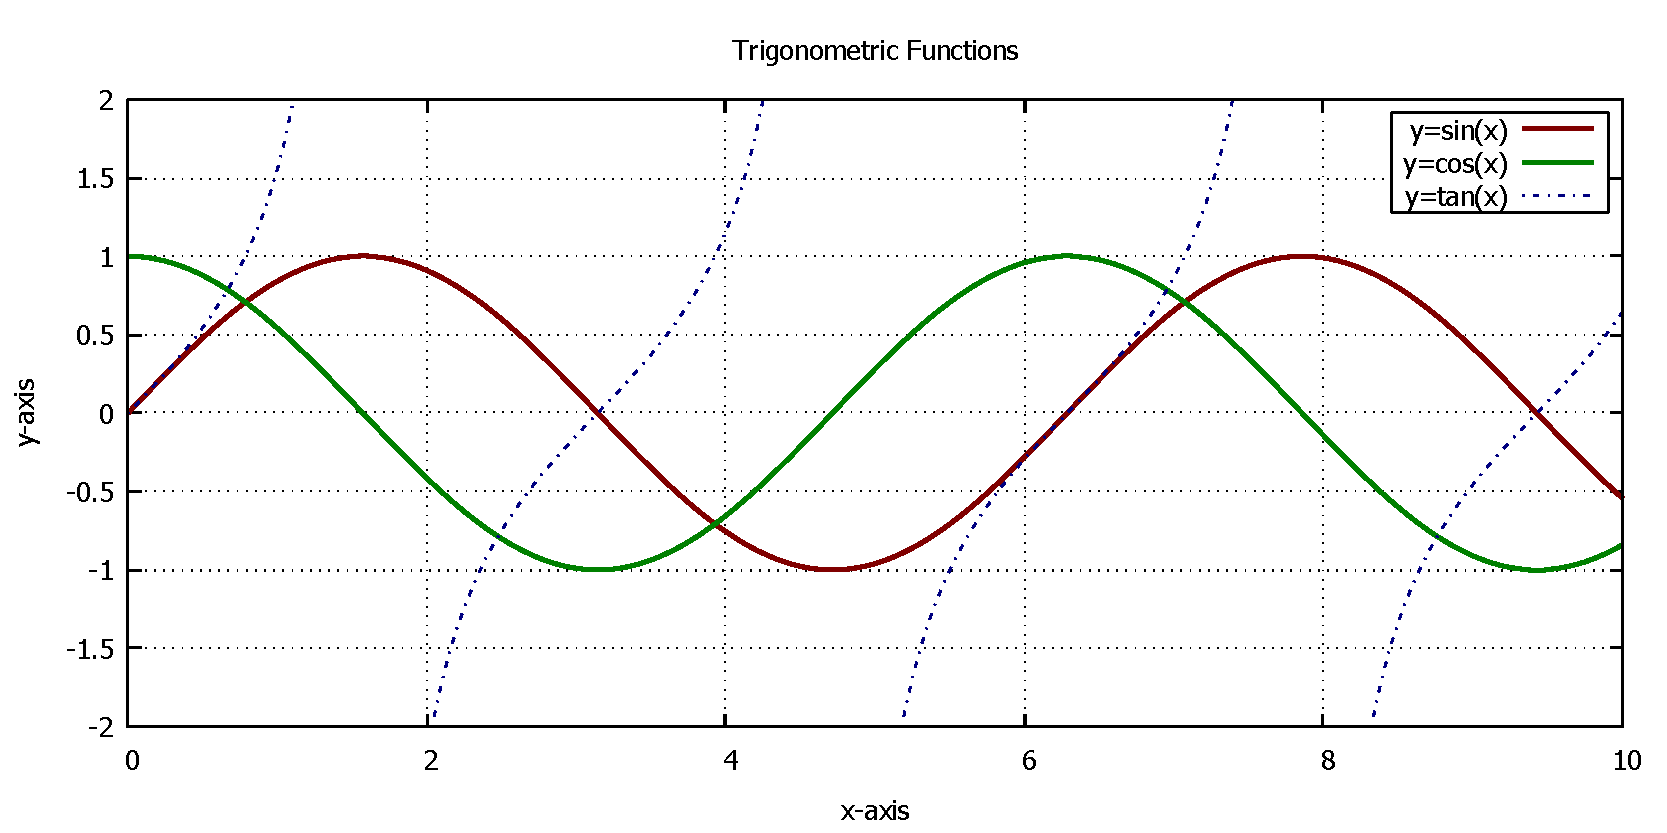
\includegraphics[width=0.80\textwidth]{Plots/TrigFunctions.pdf}
	\caption{Trigonometric Functions}
	\label{fig:TrigFunctions}
\end{figure}
\newline
You can produce this plot yourself using the function \texttt{demoTrigFunctions} which is implemented in the file \texttt{Demos.cpp}. This file contains a couple of demos how to use the \texttt{GNUPlotter} class and is distributed along with the library. Once you have a GNUPlot window open that shows your plot, you can use GNUPlot's GUI to export the plot into various formats for later inclusion into documents, as has been done for this document.

% make subsections for linetypes, pointtypes, dashpatterns, graphcolors

\section{The GNUPlot Input Files}
It has been mentioned, that the class relies on GNUPlot's mechanism to read batchfiles with commands and datafiles. For certain kinds of more exotic and specialized plots, we actually need to have an idea of the structure of these files and how GNUPlot interprets them.

\subsection{The Commandfile}
The commandfile is a plain textfile that contains all the commands that should be sent to GNUPlot, one command on each line. The example code for plotting the trigonometric functions above has created a file \texttt{"E:/Temp/gnuplotCommands.txt"} (as specified in the member variable \texttt{commandPath}). Here is a partial listing of the file:
\begin{verbatim}
# Custom Settings:
set title "Trigonometric Functions"
set key opaque box
set xlabel "x-axis"
set ylabel "y-axis"
set terminal wxt size 800,400
set xrange[0:10]
set yrange[-2:2]
set lt 1 lc rgb "#800000"
set lt 2 lc rgb "#008000"
set lt 3 lc rgb "#000080"
set lt 3 dt (1,8,5,8)

# Plotting:
plot \
'E:/Temp/gnuplotData.dat' i 0 u 1:2 w lines lw 2 t "y=sin(x)",\
'E:/Temp/gnuplotData.dat' i 0 u 1:3 w lines lw 2 t "y=cos(x)",\
'E:/Temp/gnuplotData.dat' i 0 u 1:4 w lines lw 1 t "y=tan(x)"
\end{verbatim}
In the \texttt{Custom Settings} section, you find commands that correspond to the various function calls in the C++ code listing. For example, the call \texttt{p.setTitle("Trigonometric Functions");} has generated the line \texttt{set title "Trigonometric Functions"} in the commandfile. The \texttt{p.setLegends("y=sin(x)", "y=cos(x)", "y=tan(x)"); } call has generated the line \texttt{set key opaque box}. This correspondence is kinda non obvious, but the explanation is, that the call just notices that legends should be displayed at all and tells GNUPlot \emph{how} to display them but \emph{what} will be written into them is deferred to the \texttt{plot} call. For the following commands, you will probably recognize the correspondence to the calls in the C++ code more easily. The \texttt{set lt} commands deserve a closer look: they set up the properties of the graphs in terms of an indexed \texttt{linetype} which is abbreviated as \texttt{lt}. Here, \texttt{lc} specifies the \texttt{linecolor} and \texttt{dt} the \texttt{dashtype} for the graph with the index given after the \texttt{lt} option. Dashtypes are specified by a sequence of numbers which alternately determine a lengths for solid line segments and empty space segments. The final call of \texttt{p.plotFunctions(N, xMin, xMax, &sin, &cos, &tan);} results in the \texttt{Plotting} section which contains only the actual \texttt{plot} command (but that command has been distributed over 4 lines for clarity). This very important command tells GNUPlot where it should get the data from and how it should interpret and present it. The second to last call \texttt{p.setGraphStyles("lines lw 2", "lines lw 2", "lines lw 1");} did not generate a command. Instead, it is used to control some options in the subsequent \texttt{plot} command. It's done that way because certain options, namely the plotting styles for the different graphs, can't be controlled by a \texttt{set} command before plotting but instead must be specified inside the \texttt{plot} command. In this example, we specify that we want to plot the graphs with GNUPlot's \texttt{lines} plotting style with a linewidth \texttt{lw} of \texttt{2} for graphs 1 and 2 and a linewidth of \texttt{1} for graph 3. In the actual commandfile, there is an additional third section \texttt{Default Settings} that precedes the \texttt{Custom Settings} section. This section contains commands that will always be added to the commandfile by default, so as to control the default appearance of plots. If you want to customize these default settings, you may edit the member function \texttt{addDefaultCommands} of the \texttt{GNUPlotter} class which is responsible for generating these default commands and is called from the constructor of the class.

% old version:
%The first line tells GNUPlot use display coarse grids for the x- and y-axis. The alert reader may notice, that there was no corresponding call in the code above - this setting for the grids is a default setting that the \texttt{GNUPlotter} class always adds to the start of the commandfile. I happen like plots with grids more, but GNUPlot plots without them by default, so I always add that line to override GNUPlot default behavior. If you want to get rid of it, you may comment or delete the line
%\begin{verbatim}
%setGrid();
%\end{verbatim}
%in the constructor of the \texttt{GNUPlotter} class. There, you may also add more function calls if you like to define your own default behavior. For each of the next commands, you can find a corresponding function call in the C++ code above. 
%
%As you can see, some of the styling options, such as the axis ranges and labels, have to be done \emph{before} the \texttt{plot} command via the various \texttt{set} commands, but some other styling options, such as the colors for the graphs, the line thicknesses or the legends are specified \emph{inside} the \texttt{plot} command itself. That's a bit inconvenient but it's just the way GNUPlot's syntax works and the \texttt{GNUPlotter} class takes care of that. 

\subsection{The Datafile}
GNUPlot datafiles contain the actual data that should be plotted. There are different possibilities for how the data can be formatted. The simplest one is probably to use plain ASCII textfiles where each datapoint is represented as a line and the different dimensions of the datapoint are separated by whitespaces. This is the way, this class does it. The first 4 of lines of our example datafile \texttt{E:/Temp/gnuplotData.dat} look like:
\begin{verbatim}
0.00000000e+00  0.00000000e+00  1.00000000e+00  0.00000000e+00 
5.00000000e-02  4.99791693e-02  9.98750260e-01  5.00417084e-02 
1.00000000e-01  9.98334166e-02  9.95004165e-01  1.00334672e-01 
1.50000000e-01  1.49438132e-01  9.88771078e-01  1.51135218e-01 
\end{verbatim}
and so it goes on and on and on. The first column represents the x-axis, the second column are the y-values of the \texttt{sin} function, the third column are the \texttt{cos} values and the fourth are the \texttt{tan} values. But how does GNUPlot know this? The answer to this lies in the options of the \texttt{plot} command. Consider the line
\begin{verbatim}
'E:/Temp/gnuplotData.dat' i 0 u 1:2 w lines lw 2 t "y=sin(x)",\
\end{verbatim}
from the commandfile (which you have seen already above). This is actually a shorthand syntax for:
\begin{verbatim}
'E:/Temp/gnuplotData.dat' index 0 using 1:2 with lines linewidth 2 title "y=sin(x)",\
\end{verbatim}
It tells GNUPlot, that for the first graph in the plot (because it's the first paramater in the \texttt{plot} command), it shall use the dataset with \texttt{index 0} from the datafile \texttt{E:/Temp/gnuplotData.dat} and use the first column as x-axis and the second column as y-axis via \texttt{using 1:2}. The option \texttt{with lines linewidth 2} means, that the datapoints shall be connected by lines which have a thickness of \texttt{2}. The option \texttt{title "y=sin(x)"} sets the legend for the graph that appears in the upper right corner. In this example, there is only one single dataset in the file - if there would be more than one, the subsequent datasets would be separated from each other by a double blank line. The next two lines in the commandfile are analogous:
\begin{verbatim}
'E:/Temp/gnuplotData.dat' i 0 u 1:3 w lines lw 2 t "y=cos(x)",\
'E:/Temp/gnuplotData.dat' i 0 u 1:4 w lines lw 1 t "y=tan(x)"
\end{verbatim}
and tell GNUPlot to use columns 1 and 3 as x- and y-axis values for a second graph, and columns 1 and 4 for a third graph. This is the default behavior of the \texttt{GNUPlotter} class to handle the datasets: interpret the first column as x-axis values and the subsequent columns as y-axis values for different graphs in the same plot, all to be plotted using the \texttt{lines} plotting style. As a special case, if there's only one single column, it will be interpreted as y-axis values to be plotted against an implicit x-axis given by the index. Sometimes you will want to plot datasets which do not all share the same x-axis values. In this case, a simple function call like \texttt{plotFunctions} will not be suitable. Instead, we need to dig deeper into the \texttt{GNUPlotter} class and access a lower level of control, where we explicitly add data to the datafile and also explicitly tell the plotter how to interpret it. As an example, consider the following code:
\begin{verbatim}
GNUPlotter p;
p.addDataFunctions(501, 0.0, 5.0, &square);
p.addDataFunctions(6,   0.0, 5.0, &square);
p.addGraph("index 0 using 1:2 with lines lw 2 lc rgb \"#808080\" notitle");
p.addGraph("index 1 using 1:2 with points pt 7 ps 1.2 lc rgb \"#000000\" notitle");
p.plot();
\end{verbatim}
which is taken from the function \texttt{demoSquare}. Here, \texttt{p.addDataFunctions(501, 0.0, 5.0, \&square)} tells the plotter \texttt{p} to add functional data of the function \texttt{square}, which just returns the argument squared, in the range from \texttt{0} to \texttt{5} using \texttt{501} sample values. The line \texttt{p.addDataFunctions(6, 0.0, 5.0, \&square)} adds a second dataset to the datafile, using the same function but this time using only 6 sample values, which in this case, are the integers \texttt{0,...,5}. With the two \texttt{addGraph} calls, we then tell the plotter to use the densely sampled dataset for a graph that connects the datapoints with straight lines and the dataset, that has been sampled only the integers, shall be shown as points (\texttt{pt 7 ps 1.2} means to use pointtype 7, which are filled circles, with pointsize 1.2 - refer to the GNUPlot user manual for more details). Finally calling \texttt{plot} actually invokes GNUPlot. The resulting plot is shown in Figure \ref{fig:Square}.
\begin{figure}[h!]
	\centering
  	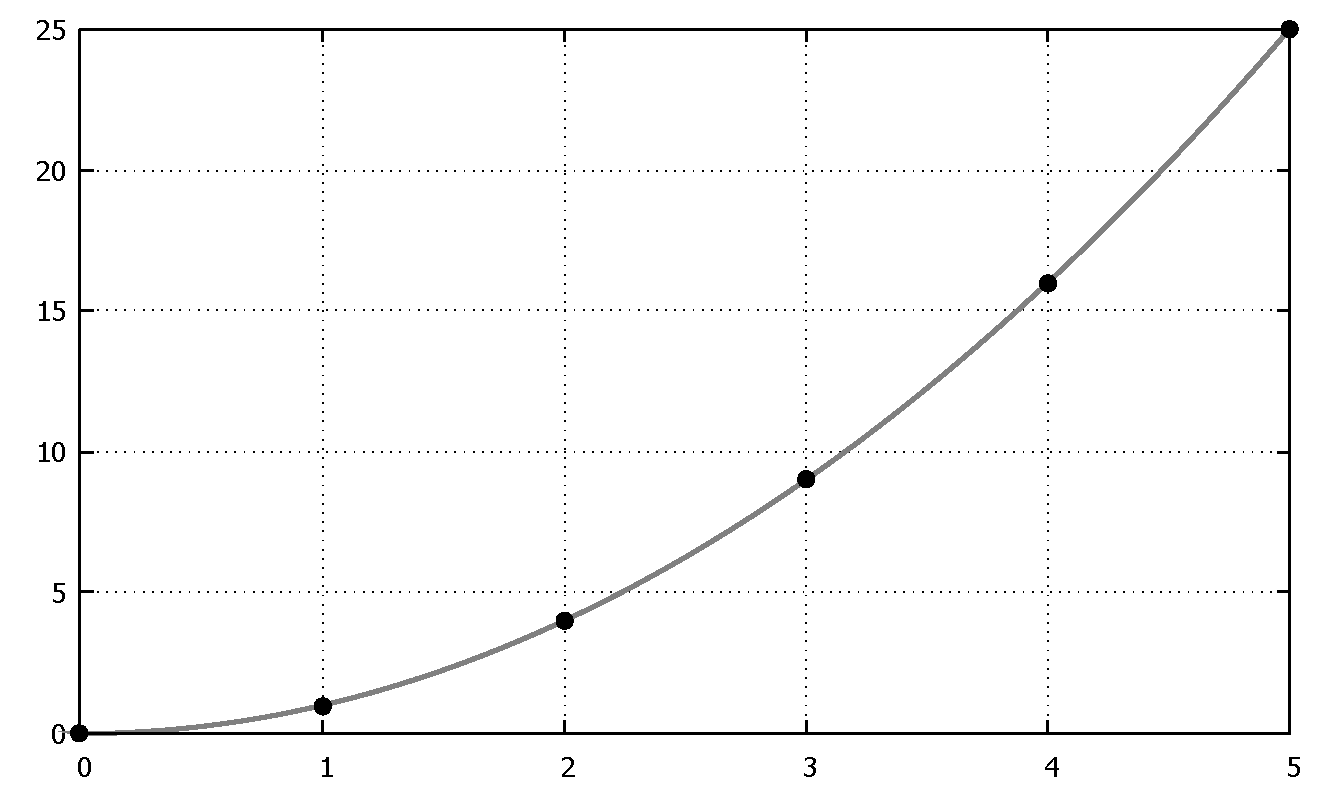
\includegraphics[width=0.60\textwidth]{Plots/Square.pdf}
	\caption{Square function - continuous and for integers}
	\label{fig:Square}
\end{figure}
The gray line is the graph for the densely sampled (i.e. pseudocontinuous) dataset and the black points are the graph of the sparsely sampled dataset that produces datapoints only for integer x-values. A function call like \texttt{plotFunctions} essentially just encapsulates this adding of data to the datafile and adding the graphs and finally invoking GNUPlot. 

\subsubsection{Interpretation of Multicolumn Datasets}
Interpreting the first column of each dataset as x- and subsequent columns as y-values for different graphs is the default behavior but by no means the only way that the data can be interpreted. For example, you could have 3 columns of data, the first one representing x-axis values, the second one representing y-axis values and the third one representing an uncertainty in the y-values (for example, due to measurement imprecision) which should be shown in the graph as errorbars. You may also have a fourth column to have different uncertainties in positive and negative direction. You may also have a fifth and sixth column to have positive and negative uncertainties for the x-values as well. GNUPlot offers various plotting styles to visualize such things and in order to make use of them, you need to be able to tell GNUPlot, how the data columns are to be interpreted. Some of these plotting styles are shown in Figure \ref{fig:PlottingStyles}.
\begin{figure}[h!]
	\centering
  	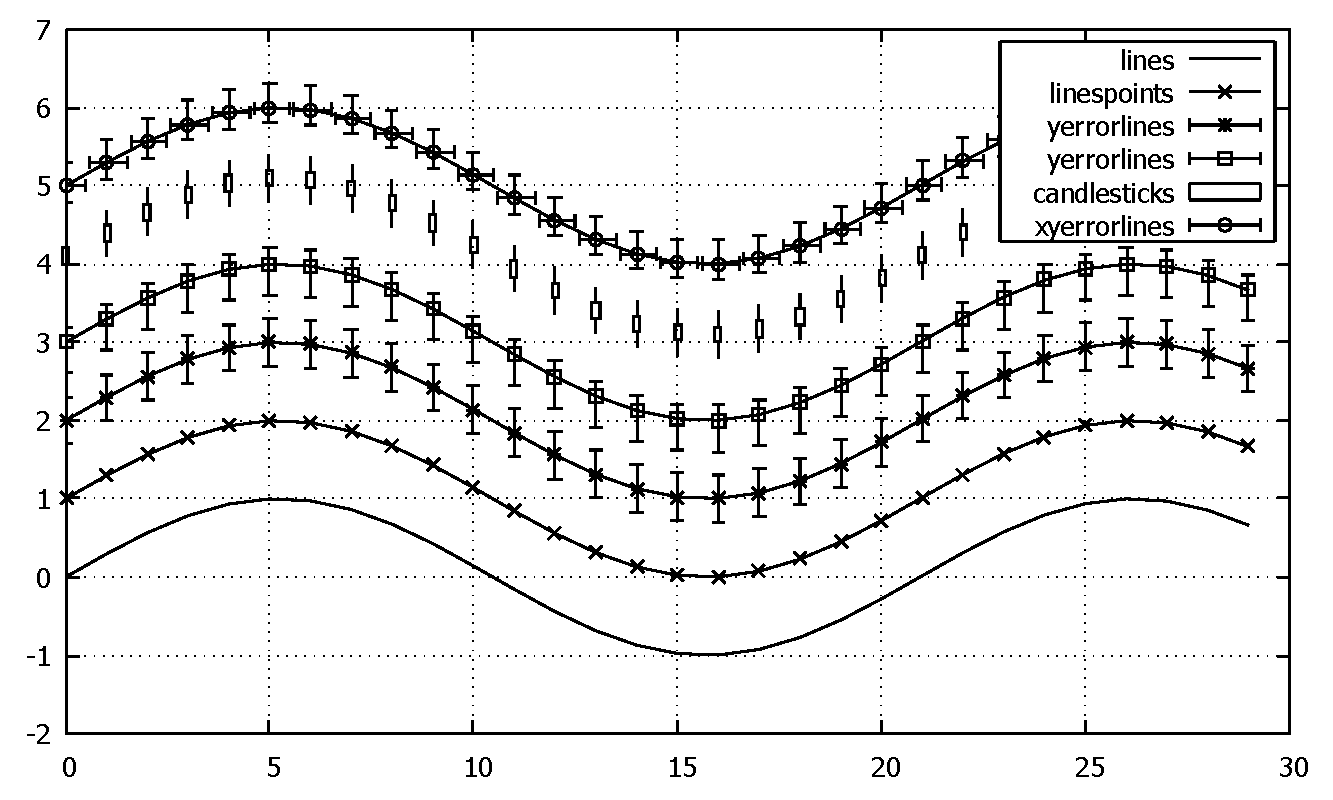
\includegraphics[width=0.60\textwidth]{Plots/PlottingStyles.pdf}
	\caption{Plotting Styles}
	\label{fig:PlottingStyles}
\end{figure}
This plot was produced by the function \texttt{demoPlottingStyles} from the collection of demos. GNUPlot offers many more plotting styles. Refer to its user manual for more about this.
% make subsection for plotting styles

%To reiterate: the addCommand function directly adds a command to the command file whereas the addGraph function stores a string that will be passed later in the actual plot command. 

\subsubsection{Blocked Datasets}
It was mentioned that individual datasets in a datafile are separated by double blank lines. You may wonder why a single blank line doesn't suffice. The answer is that single blank lines are used to separate blocks of data within a single dataset. Subdividing datasets into blocks is relevant for the correct interpretation of 3-dimensional data which will be subject of the next section. To add datasets that are subdivided into blocks, the function:
\begin{verbatim}
template <class T>
void addData(const vector<vector<vector<T>>>& d);
\end{verbatim}
can be used. It provides the most general way to add a dataset to the datafile. It takes a doubly nested \texttt{std::vector} of values (of a templated type \texttt{T} which may be either \texttt{float}, \texttt{double} or \texttt{int}). In this nested vector, the outermost index runs over the blocks, the middle index runs over the lines in each block and the innermost index over the columns in each line.

\subsubsection{Matrix Data}
GNUPlot can also interpret data in matrix form. In GNUPlotCPP, matrix datasets are passed as an array of \texttt{x}-values, an array of \texttt{y}-values and a 2D array of \texttt{z}-values. These arrays are written into the datafile in the following tabular format:
\begin{verbatim}
N+1   x[0]    x[1]    ... x[N]
y[0]  z[0][0] z[1][0] ... z[N][0]
y[1]  z[0][1] z[1][1] ... z[N][1]
...     ...     ...   ...   ...
y[M]  z[0][M] z[1][M] ... z[N][M] 
\end{verbatim}
The \texttt{N+1} value in the upper left corner is actually irrelevant in case of plain text datafiles, but it is important for binary data formats where the number of columns can't be inferred by parsing the text. With the member function
\begin{verbatim}
template <class T>
void addDataMatrix(int Nx, int Ny, T *x, T *y, T **z);
\end{verbatim}
you may add such matrix datasets to the datafile. The correspondence between the array lengths \texttt{Nx, Ny} and the \texttt{N,M} variables in the schematic view above is given by: \texttt{N=Nx-1, M=Ny-1}. For a plot that uses matrix data, the option \texttt{nonuniform matrix} has to be incorporated into the \texttt{plot} or \texttt{splot} command, right after the index of the dataset. Unlike regular datasets, matrix datasets may be separated by single blank lines in GNUPlot. Although GNUPlotCPP actually separates matrix datasets also by double blank lines, the mere fact that this is potentially possible may break GNUPlotCPP's dataset indexing when there are multicolumn datasets before matrix datasets. So, if you want to use matrix datasets and regular multiblock datasets in a single datafile, you need to add the matrix datasets \emph{first}. The same dataset can also be represented by regular $x,y,z$ triplets that are suitably arranged as blocks. The matrix data table above corresponds to the triplet dataset:
\begin{verbatim}
x[0] y[0] z[0][0]    1st block
x[0] y[1] z[0][1]
...  ...    ...
x[0] y[M] z[0][M]

x[1] y[0] z[1][0]    2nd block
x[1] y[1] z[1][1]
...  ...    ...
x[1] y[M] z[1][M]

...more blocks...

x[N] y[0] z[N][0]    (N+1)th block
x[N] y[1] z[N][1]
...  ...    ...
x[N] y[M] z[N][M] 
\end{verbatim}
which can be added in this format to the datafile using:
\begin{verbatim}
template <class T>
void addDataGrid(int Nx, int Ny, T *x, T *y, T **z);
\end{verbatim}
However, it is not really recommended to do it that way because this is a highly redundant way to represent the data and therefore bloats the size of the datafile unnecessarily. Specifically, as \texttt{N} and \texttt{M} become large, the savings in storage requirements of the matrix format compared to the triplet format approach a factor of 3. Therefore, the matrix format should be preferred, whenever possible.
The \texttt{demoMatrixData} function gives example code, how to use the matrix format. It plots the data reduction as function of \texttt{N} and \texttt{M}, so it shows not only \emph{how} the matrix format is used, but also gives a motivation \emph{why}.


%\section{Plotting Styles}
%\subsection{Linetypes}
%\subsection{Pointtypes}


\section{3D Plots}
So far, we have only seen 2-dimensional plots but GNUPlot may also create 3-dimensional plots. GNUPlot itself has a different command for 3D plots: instead of using \texttt{plot}, the command \texttt{splot} is used (I guess, it's an abbreviation of surface plot). In GNUPlotCPP, this is reflected by using the \texttt{plot3D} member function of \texttt{GNUPlotter} instead of \texttt{plot}. A dataset for a 3D object is typically represented in a way in which each datapoint is represented by 3 coordinate values - so, a datapoint is a triple of $x,y,z$ coordinate values. It's also possible to use coordinate systems other than the cartesian, such as spherical and cylindrical coordinates. Anyway, in each case, a datapoint is a triple of coordinate values. So, in order to create 3D plots, we should create a datafile with 3 columns and then use the \texttt{plot3D} function to initiate the actual plotting. In cases where the intrinsic dimensionality of our object is 2 (such as surfaces), we will also need to take care of proper subdivision of the dataset into blocks. As with 2D plots, for some specific types of 3D plots, convenience functions are available which wrap the data generation and GNUPlot invocation.

\subsection{Parametric Curves in Space}
A simple example for a 3D plot is a parametric curve in space. Such curves are typically created by a set of 3 equations that associate $x$-, $y$- and $z$-values to an independent parameter (typically $t$) which goes through a range of values. The intuition here is, that $t$ represents a time variable and the 3 equations give the position of a moving point/object at a particular time instant $t$. For example, a helical curve could be represented by:
\begin{equation}
	x(t) = \cos(t), \; y(t) = \sin(t), \; z(t) = t \qquad t \in [0, 50]
\end{equation}
The parameter $t$ traverses the range of values from $0$ to $50$ and for each value of $t$, a triple of $x,y,z$ coordinate values is produced by the 3 formulas. Code for plotting such a helix with GNUPlotCPP could look like:
\begin{verbatim}
static const int N = 1001;                  // number of datapoints
double tMin = 0;                            // minimum value for parameter t
double tMax = 50;                           // maximum value for parameter t
double t[N], x[N], y[N], z[N];              // arrays for t,x,y,z
GNUPlotter::rangeLinear(t, N, tMin, tMax);  // fill t-array with equidistant values
for(int i = 0; i < N; i++)
{
  x[i] = cos(t[i]);                         // x(t) = cos(t)
  y[i] = sin(t[i]);                         // y(t) = sin(t)
  z[i] = t[i];                              // z(t) = t
}
GNUPlotter p;                               // create plotter object
p.addDataArrays(N, x, y, z);                // pass the data to the plotter
p.addCommand("set view 60,320");            // set up perspective
p.plot3D();                                 // invoke GNUPlot
\end{verbatim}
This code is taken from the \texttt{demoHelix} function and it produces the plot of figure \ref{fig:Helix}.
\begin{figure}[h!]
	\centering
  	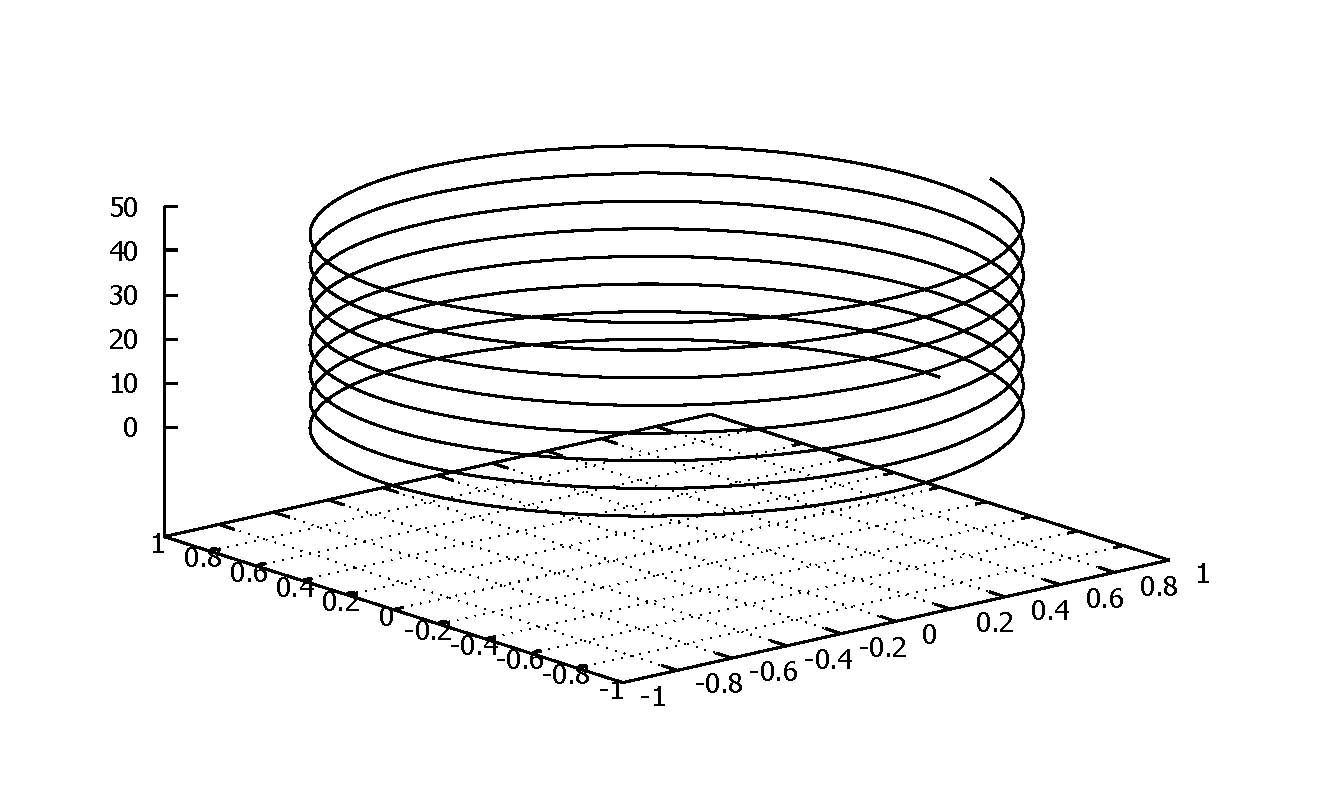
\includegraphics[width=0.60\textwidth]{Plots/Helix.pdf}
	\caption{Helix}
	\label{fig:Helix}
\end{figure}
It should be noted that the the curve is intrinsically just a one dimensional object - there's just a single independent variable and the whole curve could be deformed into a straight line.


\subsection{Parametric Surfaces in Space}
It is also possible to plot 2-dimensional surfaces in a 3D plot. Here, the intrinsic dimensionality of our object is 2 and we need 2 independent parameters to describe it via equations. Typically $u$ and $v$ are used to denote these parameters. For example, the surface of a torus with major radius $R$ and minor radius $r$ can be represented by the 3 parametric equations:
\begin{equation}
	x(u,v) = \cos(u) (R+r \cos(v)), \; y(u,v) = \sin(u) (R+r \cos(v)), \; z(u,v) = r \sin(v) \qquad u,v \in [0, 2\pi]
\end{equation}
The code for plotting such a torus with GNUPlotCPP could look like:
\begin{verbatim}
double R = 2.0;                                // major radius
double r = 0.5;                                // minor radius
static const int Nu = 41;                      // number of grid lines around the major radius
static const int Nv = 21;                      // number of grid lines around the minor radius
double u[Nu], v[Nv];                           // arrays for parameters u and v
GNUPlotter::rangeLinear(u, Nu, 0.0, 2*M_PI);   // fill u-array with equidistant values
GNUPlotter::rangeLinear(v, Nv, 0.0, 2*M_PI);   // fill v-array with equidistant values
vector<vector<vector<double>>> d;              // doubly nested vector of data
d.resize(Nu);                                  // we have Nu blocks of data
for(int i = 0; i < Nu; i++)                    // loop over the data blocks
{
  d[i].resize(Nv);                             // each block has Nv lines/datapoints
  for(int j = 0; j < Nv; j++)                  // loop over lines in current block
  {
    d[i][j].resize(3);                         // each datapoint has 3 columns/dimensions
    d[i][j][0] = cos(u[i]) * (R+r*cos(v[j]));  // x = cos(u)*(R+r*cos(v))
    d[i][j][1] = sin(u[i]) * (R+r*cos(v[j]));  // y = sin(u)*(R+r*cos(v))
    d[i][j][2] = sin(v[j]) * r;                // z = sin(v)*r
  }
}
GNUPlotter p;                                  // create plotter object
p.addData(d);                                  // pass the data to the plotter         
p.addCommand("set hidden3d");                  // don't draw hidden lines
p.addCommand("set view 20,50");                // set up perspective
p.addCommand("set lmargin 0");                 // margin between plot and left border
p.addCommand("set tmargin 0");                 // margin between plot and top border
p.addCommand("set ztics 0.5");                 // density of z-axis tics
p.plot3D();                                    // invoke GNUPlot
\end{verbatim}
This code is taken from the function \texttt{demoTorus}. Note the use of our most general data adding member function:
\begin{verbatim}
template <class T>
void addData(const vector<vector<vector<T>>>& d);
\end{verbatim}
here, that takes a dataset which is subdivided into blocks. For 2-parametric, 3-dimensional data, the dataset should be divided into blocks where each block corresponds to a particular value of the first parameter ($u$ in this case). Organizing the dataset this way ensures, that not only the lines between subsequent datapoints are drawn, but also the other 2 edges of the quadrangles that make up our 2-dimensional surface grid of our 3-dimensional shape. The code above produces the plot in figure \ref{fig:Torus}. In this example, our 2D surface is the surface of a solid 3D object, but that doesn't need to be the case.
\begin{figure}[h!]
	\centering
  	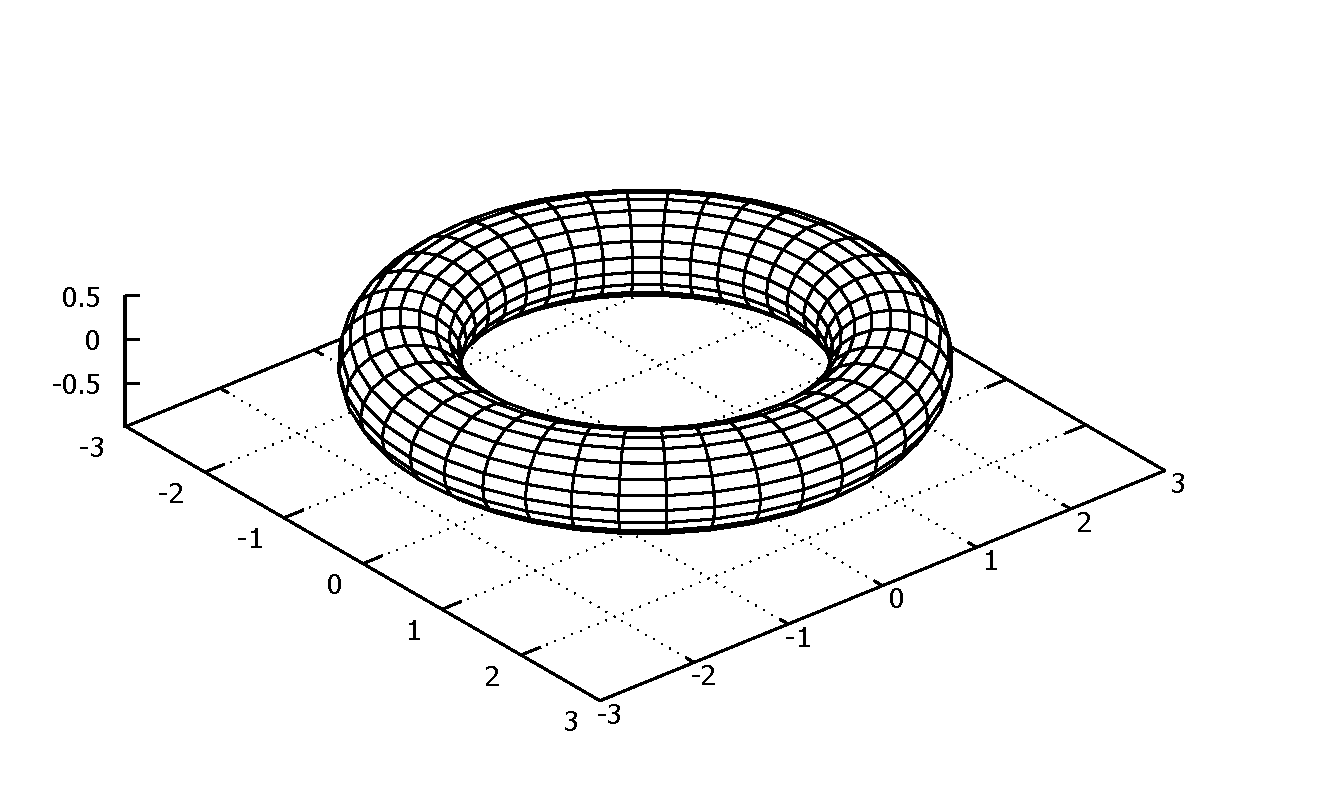
\includegraphics[width=0.60\textwidth]{Plots/Torus.pdf}
	\caption{Torus}
	\label{fig:Torus}
\end{figure}

\subsection{Bivariate Functions}
Another important type of 3D plots are functions of 2 independent variables (a.k.a. bivariate functions) where the function value is plotted as a height value above an $xy$-plane. As an example, consider the bivariate Gaussian distribution (with zero mean and unit covariance matrix) given by:
\begin{equation}
	f(x,y) = e^{-(x^2+y^2)}
\end{equation}
In C++ code, you could implement this function like:
\begin{verbatim}
double gauss2D(double x, double y)
{
  return exp(-(x*x+y*y)); 
}
\end{verbatim}
Having this function in place, you could plot it with GNUPlotCPP with the following code:
\begin{verbatim}
GNUPlotter p;
p.addCommand("set hidden3d");
p.addCommand("set ztics 0.2");
p.setGraphColors("000000", "000000"); // paint both sides black
p.plotBivariateFunction(31, -2.0, 2.0, 31, -2.0, 2.0, &gauss2D);
\end{verbatim}
Here, we plot it for x- and y- range values from \texttt{-2} to \texttt{2} using \texttt{31} sample values along each direction. This code is taken from \texttt{demoGaussianBivariate} and produces the plot shown in figure \ref{fig:GaussianBivariate}.
\begin{figure}[h!]
	\centering
  	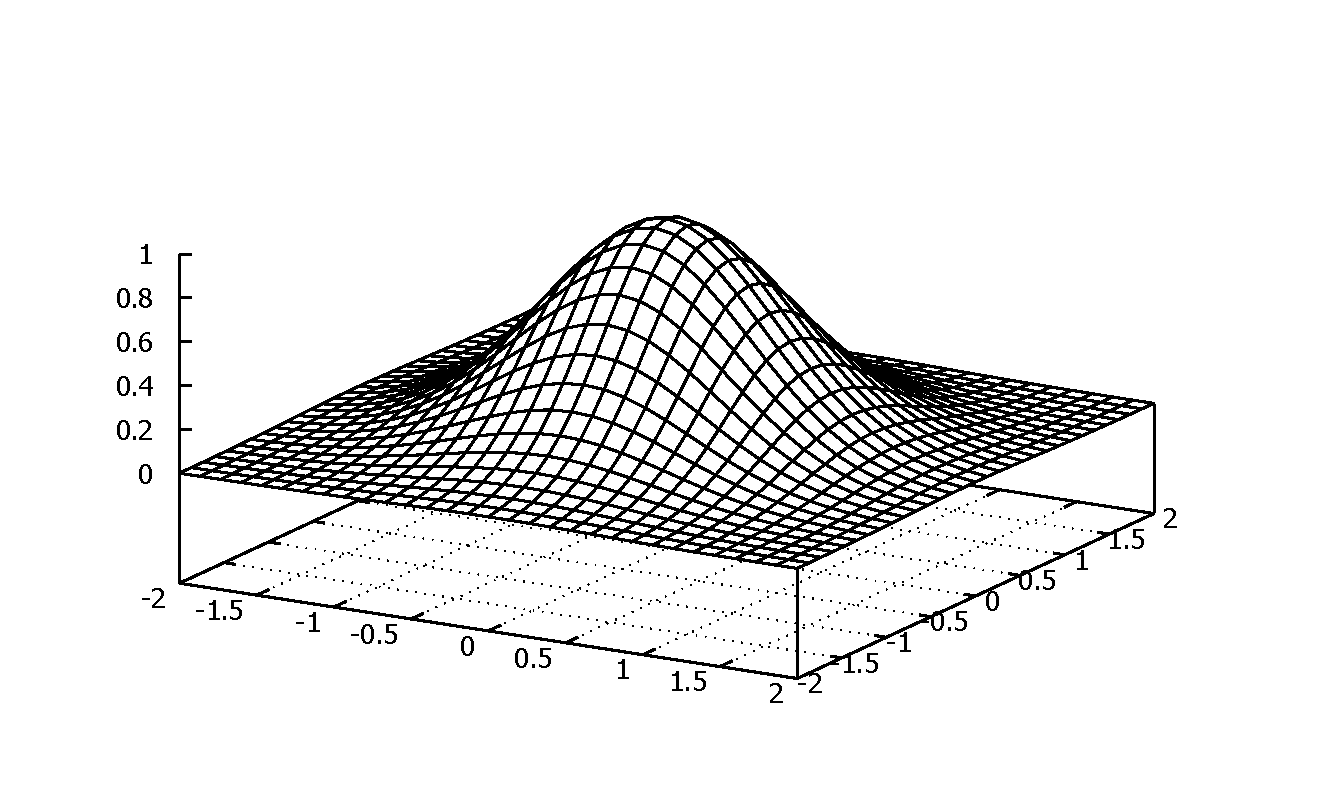
\includegraphics[width=0.60\textwidth]{Plots/GaussianBivariate.pdf}
	\caption{Bivariate Gaussian Distribution}
	\label{fig:GaussianBivariate}
\end{figure}
If you don't care about wrapping your bivariate function into a C++ function such as the \texttt{gauss2D} function shown above, or it is impractical to do so (maybe because your function has additional parameters), you could also generate the data for the x- and y-axis values and the z-axis (height) values as arrays (where the z-array is 2-dimensional, i.e. an array of pointers to 1D arrays) and use the function:
\begin{verbatim}
template <class T>
void plotSurface(int Nx, int Ny, T *x, T *y, T **z);
\end{verbatim}
Here, \texttt{x} and \texttt{y} are the arrays of the x- and y-axis values of lengths \texttt{Nx} and \texttt{Ny} respectively, and your 2 dimensional \texttt{z} array should be filled with values such that \texttt{z[i][j] = f(x[i], y[j])} where \texttt{f} is your bivariate function. Bivariate functions and datasets are the primary application of the matrix data format.

% levels of access:
%1.) call convevnience (non-member) functions plotFunctions/Arrays/etc.
%    -very quick and easy (single line of code), no customization possible
%2.) create object, setup, call plotArrays/...
%    -still quick and easy (2 lines + optional setup code), limited customizations (colors, etc.)
%3.) create object, add data, setup, call plot/plot3D (graphs will be added automatically)
%    -multiple datasets can be added, they will be interpreted automatically
%4.) create object, add data, setup, add graphs, call plot/plot3D
%    -interpretation of datasets can be controlled
%5.) create object, add data, setup, add plot/splot command manually, call invokeGNUPlot
%    -the options of the plot/splot command can be controlled


% add another example using the bivariate sinc function -> add contours, maybe make an extra section
% contourplots

\section{Examples}
Depending on the application domain, you write code for, you may need different types of data visualization. GNUPlot offers a wide variety of plotting methods and in this section, we will explore a few and show how they can be harnessed from a C++ environment with GNUPlotCPP by means of examples. The code for creating all these examples can be found in the file \texttt{Demos.cpp}. If you want to create a particular type of plot, you may refer to these examples, find one which is conceptually similar to what you have in mind and look at the code, copy/paste/edit etc. I'm myself rooted in the field of audio software development with focus on signal processing algorithms, so some of the examples might be skewed toward that application domain.

\subsection{Function Plots}
The most common type of plots is the graph of one or more functions of a single independent variable. With GNUPlotCPP, you can create such plots for example by passing an array with values of the independent variable and one or more arrays of dependent variables. 

\paragraph{Aliasing}
The plot in figure \ref{fig:Aliasing} was created by the function \texttt{demoAliasing}. It shows two continuous-time sine waves with frequencies 3 Hz and 7 Hz and samples of them which would be produced when sampling the signals at a samplerate of 10 Hz. It can be seen, that both sinusoids would lead to the exact same sequence of sampled values. This demonstrates, that a 7 Hz sinusoid would alias into a 3 Hz sinusoid when sampled at 10 Hz samplerate.
\begin{figure}[h!]
	\centering
  	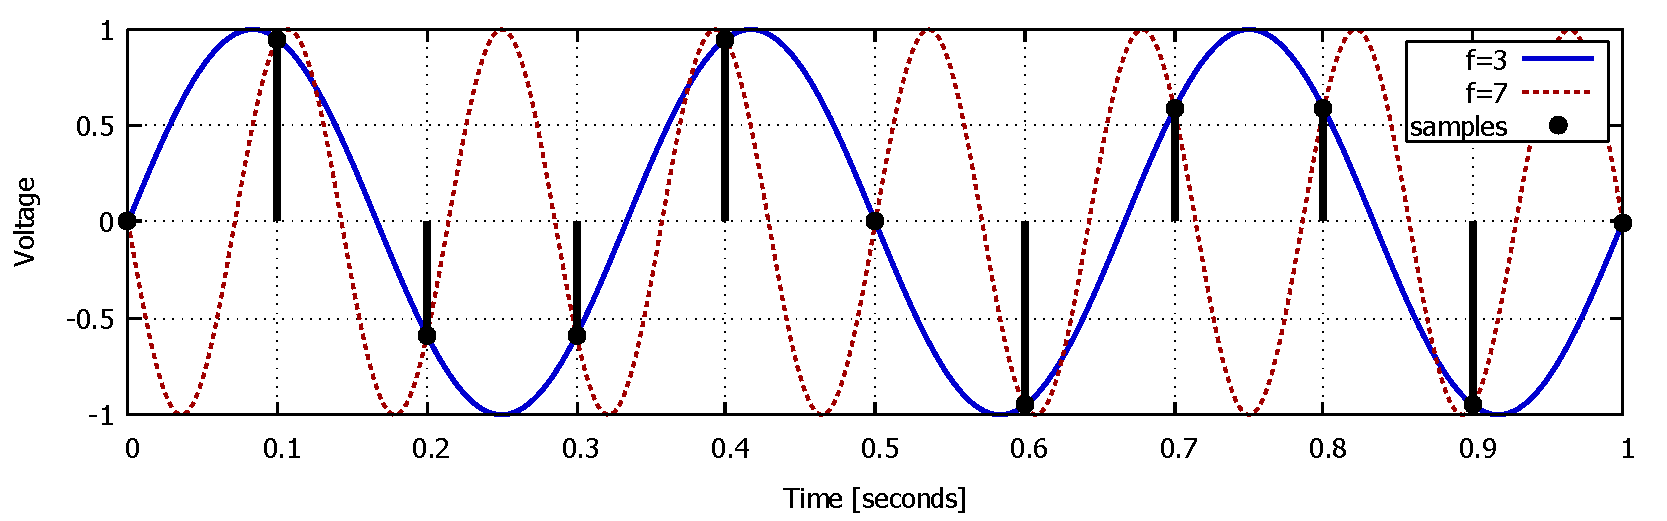
\includegraphics[width=0.80\textwidth]{Plots/Aliasing.pdf}
	\caption{Aliasing of a 7 Hz Sinusoid into a 3 Hz Sinusoid at 10 Hz samplerate}
	\label{fig:Aliasing}
\end{figure}

\paragraph{Frequency Responses}
In figure \ref{fig:ButterworthResponses} are plots of magnitude- and phase responses of Butterworth filters of orders 1-5 with a cutoff frequency of 1 kHz. The plot demonstrates the use of a logarithmic x-axis and dual y-axes, one on the left, one on the right. The plot was created with \texttt{demoFrequencyResponse}.
\begin{figure}[h!]
	\centering
  	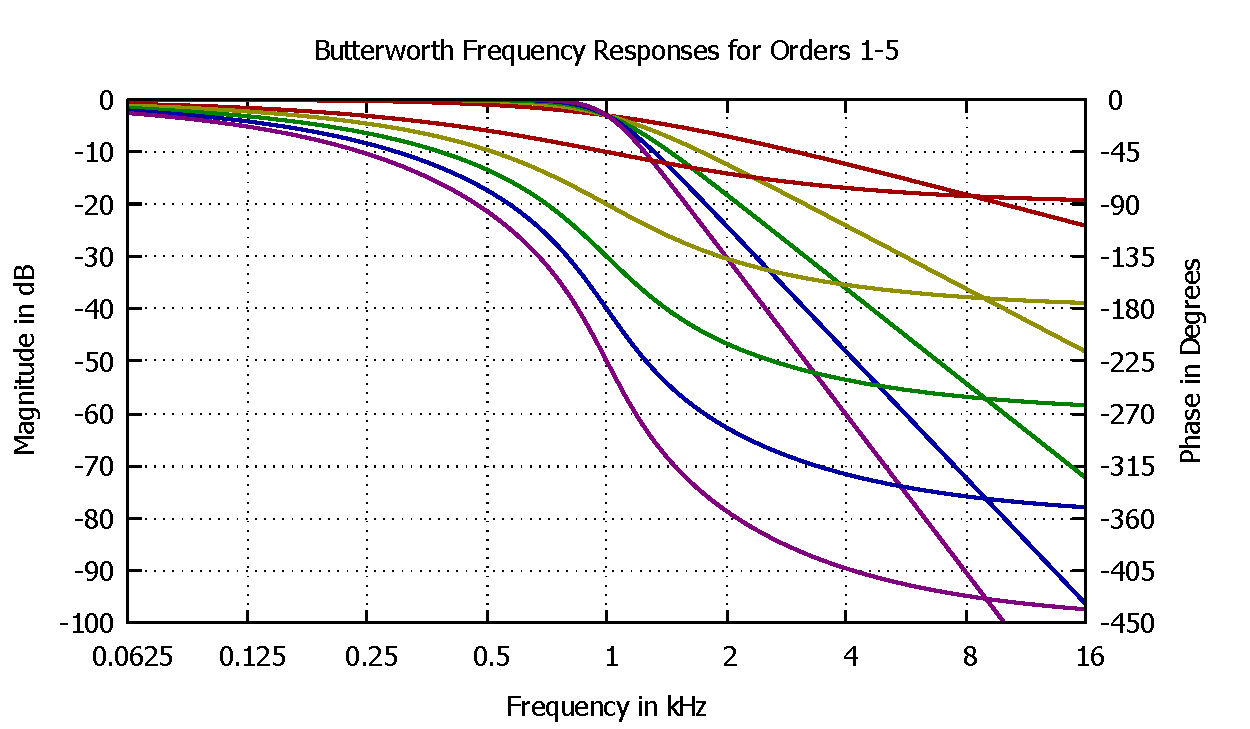
\includegraphics[width=0.60\textwidth]{Plots/ButterworthResponses.pdf}
	\caption{Frequency Resposes of Butterworth Filters}
	\label{fig:ButterworthResponses}
\end{figure}

%\subsection{Parametric Plots}
%\paragraph{Lissajous Figures}
%\paragraph{Helix}
%\paragraph{Torus}

%\subsection{Bivariate Functions}
%\paragraph{Radial Sinc Function}

\subsection{Heatmaps} 
A heatmap is another way of visualizing bivariate data, where the value of dependent variable is encoded as color. You draw the 2-dimensional plane of the 2 independent variables and each point of the plane is colored according to the function value of the dependent variable at that position. How the function values translate to colors is defined by the colormap. When 'cold' colors are chosen for low values and 'hot' colors are chosen for high values, the term 'heatmap' makes intuitive sense. Generally, the colormap should be chosen in a way that creates some sense of ordering of the colors from low to high. Sometimes it is important that the sense of ordering is preserved, when the colors are converted to grayscale for printing. This is trivially satisfied by grayscale colormaps, where a higher value directly translates to a brighter (or darker) gray value. Rainbow colormaps, on the other hand, tend to become an unordered, meaningless mess when converted to grayscale. As an example for a heatmap, consider the radial sinc function, defined by:
\begin{equation}
 sinc(r) = \frac{\sin(\pi r)}{\pi r} \quad \text{where} \quad r(x,y) = \sqrt{x^2+y^2}
\end{equation}
If we implement this function in C++ as \texttt{double sincRadial(double x, double y)}, we may plot a heatmap of that function with the following code:
\begin{verbatim}
GNUPlotter p;
p.addDataBivariateFunction(101, -5.0, 5.0, 101, -5.0, 5.0, &sincRadial);
p.setPixelSize(450, 400);
p.addCommand("set size square");                      // set aspect ratio to 1:1
p.addGraph("i 0 nonuniform matrix w image notitle");  
p.addCommand("set palette rgbformulae 30,31,32");     // colors printable as grayscale
p.plot();
\end{verbatim}
which produces the plot shown in \ref{fig:SincHeatmapPrintableColors}.
\begin{figure}[h!]
 \centering
 \begin{subfigure}[b]{0.45\textwidth}
  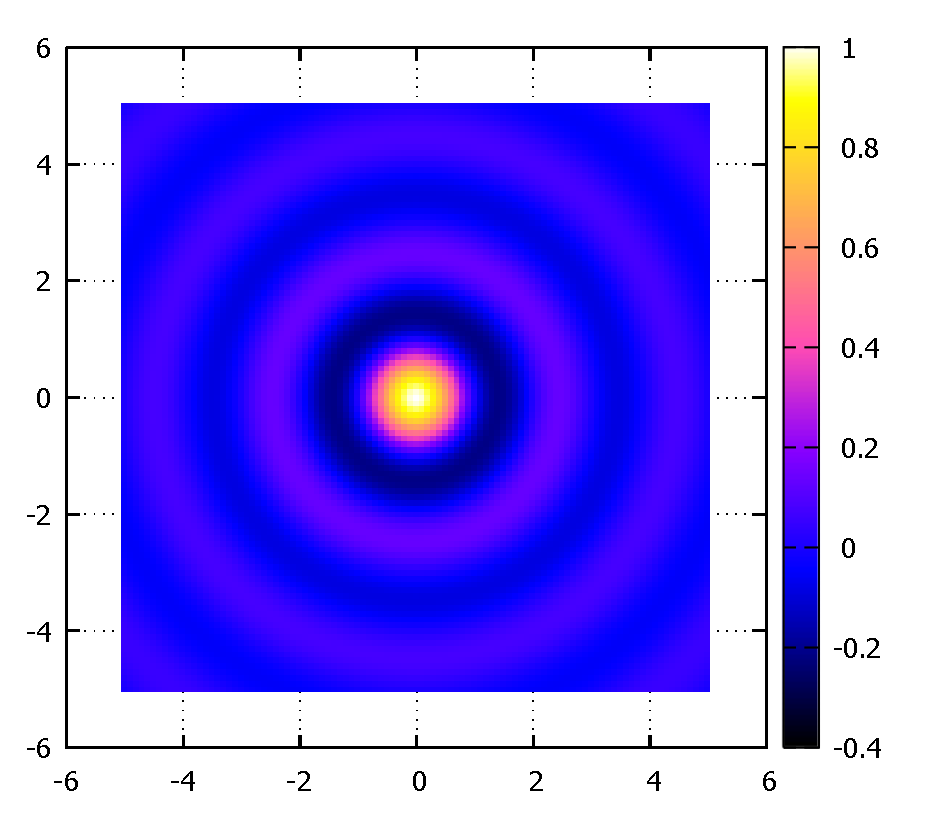
\includegraphics[width=\textwidth]{Plots/SincHeatmapPrintableColors.pdf}
  \caption{gray printable colormap}
	\label{fig:SincHeatmapPrintableColors}
 \end{subfigure}
 \begin{subfigure}[b]{0.45\textwidth}
  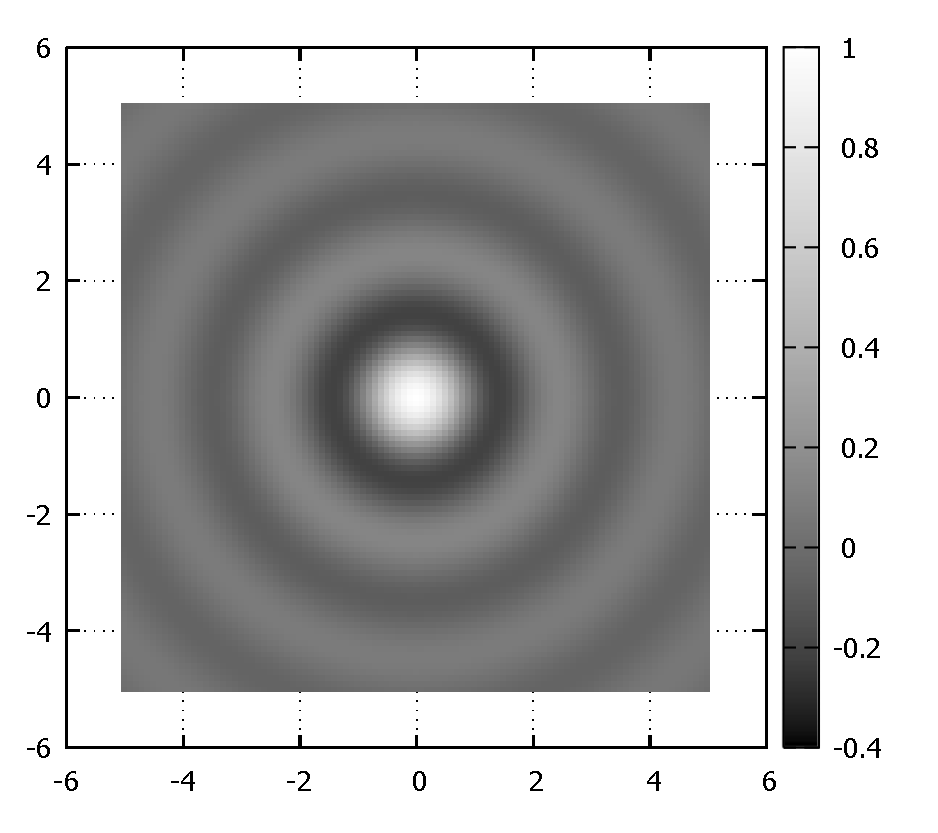
\includegraphics[width=\textwidth]{Plots/SincHeatmapGrayscale.pdf}
  \caption{grayscale colormap}
  \label{fig:SincHeatmapGrayscale}
 \end{subfigure}
 \caption{Heatmap of radial sinc function}
 \label{fig:SincHeatmap}
\end{figure}
Also shown is a heatmap which has been produced using a grayscale colormap. I suppose (but didn't verify), that the colored heatmap should print out in grayscale the same or similar to the actual grayscale heatmap. The GNUPlot manual suggests that the \texttt{palette rgbformulae 30,31,32} was made for that purpose. In the function \texttt{demoSincRadialHeatMap}, you find some commented code that you can use to experiment with various colormaps.

%\subsection{Polar Plots}
%\subsection{Parametric Curves in 2D}
%\subsection{Complex Mappings}
%\subsection{Contour Plots}
%\subsection{Direction Fields}
%\subsection{Root Locus Plots} 
%\subsection{Trajectory Plots} Lorentz Attractor...but actually, this is already covered by the helix plot
%\subsection{Histograms}
%\subsection{Scatter Plots}
%\subsection{Second x- and y-Axis}
%\subsection{Function Family Plots}
%\subsection{Multiplots} %Lissajous figure in 3D - 3 2D views and 1 3D view - a (2,2) multiplot


%Further Reading
% a large collection of demos:
%http://www.gnuplot.info/demo/


% maybe define as appendix
\section{Coding Decisions and Limitations}
In this section, I try to justify some of the weird coding decisions I made. You need to read that only if you look into the code and think to yourself: WTF?

\subsection{Use of Templates}
The plotting- and data-passing member functions are templated on the type of the data that should be plotted. In the implementation file, explicit instantiations are requested from the compiler for all datatypes that should be supported (which are \texttt{double}, \texttt{float} and \texttt{int}). This looks a bit messy but is certainly much better than writing out all the functions for all 3 types. Another alternative would have been to just implement the whole class in the header file and rely on instantiation as needed whenever your code needs a function instance for a particular type.  That would make it work for all datatypes and not just the 3 mentioned ones. But inlining the whole implementation code into your client code whenever you include the \texttt{GNUPlotter.h} file somewhere comes with its own set of problems (''multiple definition'' compiler errors and stuff), so it seemed better to have a separate implementation file and use explicit instantiations. You may notice that explicit instantiations do not exist for all templated functions. This is because some of these functions invoke others in which case only the outermost function needs an explicit instantiation. This outermost explicit instantiation triggers an instantiation cascade in the compiler such that it generates instantiations for the inner functions as well.

\subsection{Variable Argument Lists without \texttt{va\_list}}
Many of the member functions have a lot of optional parameters which default to the \texttt{null} value of the corresponding type (\texttt{nullptr} for pointers, the empty string \texttt{""} for strings, etc.). These optional parameters make it possible to pass a variable number of arguments to the functions without having to use the \texttt{va\_list, va\_arg} mechanism of C++. It was decided to not use it because it always requires an additional parameter just for the sake handling the variable argument list. It would require client code to either pass a \texttt{null} argument as last argument (which uglifies the client code) or to pass the actual number of variable arguments along (which uglifies even more and is additionally error-prone). That's why a pseudo-variable argument list mechanism was implemented which makes use of optional parameters. The disadvantage is, that the maximum number of arguments is limited, but i think, in most cases, 9 or 10 should be enough. If you really need to plot more than 9 arrays in a single plot, you probably have them in form of a 2D-array anyway and can pass them as such via \texttt{addData(int numRows, int numColumns, T **data)}.




\section{Links}

\htmladdnormallink{www.gnuplot.info/}{http://www.gnuplot.info/}
This is the official GNUPlot website. Here you find downloads for installers, sourcecode and the user manual.

\htmladdnormallink{http://gnuplot.sourceforge.net/demo/}{http://gnuplot.sourceforge.net/demo/}
A lot of demo scripts for GNUPlot. Here you can learn, how different kinds of plots can be done in GNUPlot.

\htmladdnormallink{http://www.gnuplotting.org/}{http://www.gnuplotting.org/} A blog with a lot of examples of very polished and advanced plots.

\htmladdnormallink{http://lowrank.net/gnuplot/index-e.html}{http://lowrank.net/gnuplot/index-e.html} A  tutorial which provides examples for a lot of realistic use cases.

\htmladdnormallink{http://soukoreff.com/gnuplot/}{http://soukoreff.com/gnuplot/} This site has a couple of interesting 3D plots.

\htmladdnormallink{http://ndevilla.free.fr/gnuplot/}{http://ndevilla.free.fr/gnuplot/}
Another GNUPlot programming interface for C that uses pipes (with two 3rd party ports to C++), plus interfaces for Python, Fortran and Perl





%http://soukoreff.com/gnuplot/







%Convenience vs. Flexibility
%
%One of the goals was to make the plotter as easy and convenient to use in common scenarios but to make it
%also flexible enough to allow for cuto
%
%3 Convenience levels (roughly):
%Level 1:
%-just call static functions in one-liner statement, using the default settings
%-for quick and easy plots without any customizations
%
%Level 2:
%-instantiate a GNUPlotter object, set up plotting styles and then call an appropriate plotting 
 %function on the plotter object
%-allows for customization of colors, plot-size, axes, naming of axes, legends etc. via functions such
 %as setSize, setLabels, etc.
%
%Level 3:
%-instantiate a GNUPlotter object, set up plotting styles, pass in the datasets manually, optionally
 %set up graph-styling option for each dataset, choose how data is to be interpreted, etc.
%-possibly add custom GNUPlot commands to the comannd batchfile which are not supported by wrapper 
 %functions - using the function addCommand
%-allows for plots with error-bars, etc.
%-allows to plot more than 9 functions or arrays at a time (using the more general data-adding functions)

%explain:
%-GNUPlot batchfile and datafile 
%-templates with explicit instantiations (for double, float and int)
%-limitation: it doesn't return from the plot function until you close the plot, this implies, you 
 %can only do one plot at a time
%-variable argument list (via default arguments - not via va_list -> more convenient, but sets a limit
 %on the number of arguments)
%
 %-explain that it would also be possible to use pipes


 
\end{document}
